\chapter{Ejemplos}

En este capítulo se presentará el software desde un punto de vista práctica mostrando ejemplos de uso sobre dos esculturas a las que previamente se les hicieron una TC.

Estas esculturas son las de \href{http://patrimonio3d.ugr.es/index.php/granada/escultura/item/18-inmaculada-concepcion}{\textbf{Inmaculada Concepción}} y \href{http://patrimonio3d.ugr.es/index.php/granada/escultura/item/6-san-juan-evangelista}{\textbf{San Juan Evangelista}} \ref{fig:figuras_reales}, ambas patrimonio de la Universidad de Granada y cuyos datos DICOM han sido proporcionados por el proyecto de Portal Virtual de Patrimonio de las Universidades Andaluzas, coordinado por la Universidad de Granada a quién se agradece su cesión.

\begin{figure}[H]
	\centering
	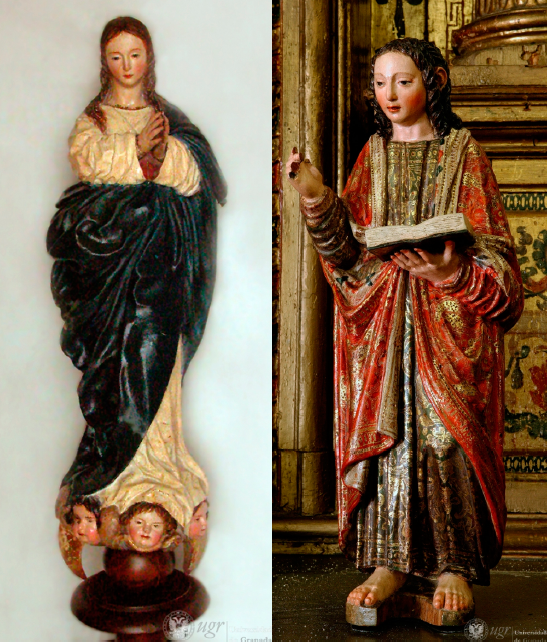
\includegraphics[width=7cm]{imagenes/figuras_reales}
	\caption{Esculturas utilizadas para realizar las pruebas. Inmaculada Concepción (izquierda) y San Juan Evangelista (derecha)}
	\label{fig:figuras_reales}
\end{figure}

\section{Presets}

Se han creado cuatro presets distintos de funciones de transferencias:

\begin{itemize}
	\item \textbf{CT-OnlyWood}: Para mostrar tan solo la madera.
	\item \textbf{CT-OnlyStucco}: Para mostrar tan solo el estuco.
	\item \textbf{CT-OnlyMetal}: Para mostrar el metal (también se ve con mucha transparencia la madera para tener una referencia de dónde se encuentra el metal).
	\item \textbf{CT-WoodSculpture}: Muestra todos los materiales. Es el utilizado al abrir el programa.
\end{itemize}

Gracias a estos se puede ver que la escultura de Inmaculada Concepción (Figura \ref{fig:inmaculada_concepcion}) no tiene objetos metálicos como pueden ser clavos en su interior. Y además, tiene una capa de estuco bastante gruesa sobre todo en el manto, la cara y las manos.

Al contrario, la escultura de San Juan Evangelista (Figura \ref{fig:san_juan_evangelista}) tiene bastante menos estuco y se pueden observar cinco clavos: dos en los pies, dos en la pierna (bastante torcidos) y uno en la cintura.

\begin{figure}[H]
	\centering
	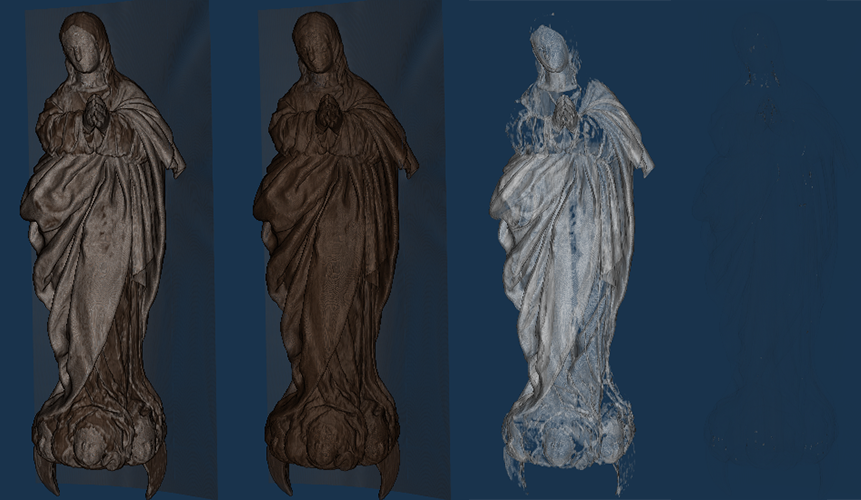
\includegraphics[width=12cm]{imagenes/inmaculada_concepcion}
	\caption{Reconstrucción volumétrica de Inmaculada Concepción usando los cuatro presets proporcionados}
	\label{fig:inmaculada_concepcion}
\end{figure}

\begin{figure}[H]
	\centering
	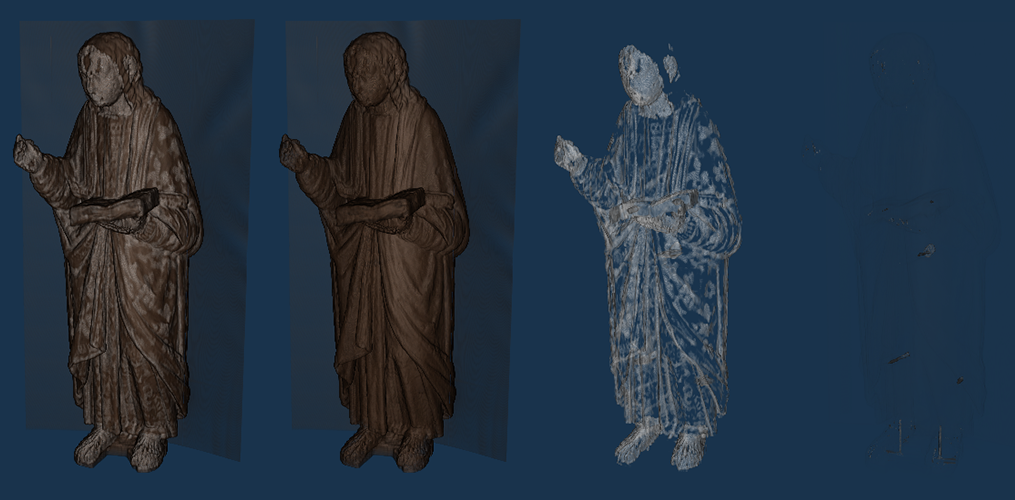
\includegraphics[width=12cm]{imagenes/san_juan_evangelista}
	\caption{Reconstrucción volumétrica de San Juan Evangelista usando los cuatro presets proporcionados}
	\label{fig:san_juan_evangelista}
\end{figure}

Se puede elegir entre estos cuatro presets o cambiar la función de transferencia usando las gráficas (Figura \ref{fig:pestana_funcion_de_transferencia}).

\begin{figure}[H]
	\centering
	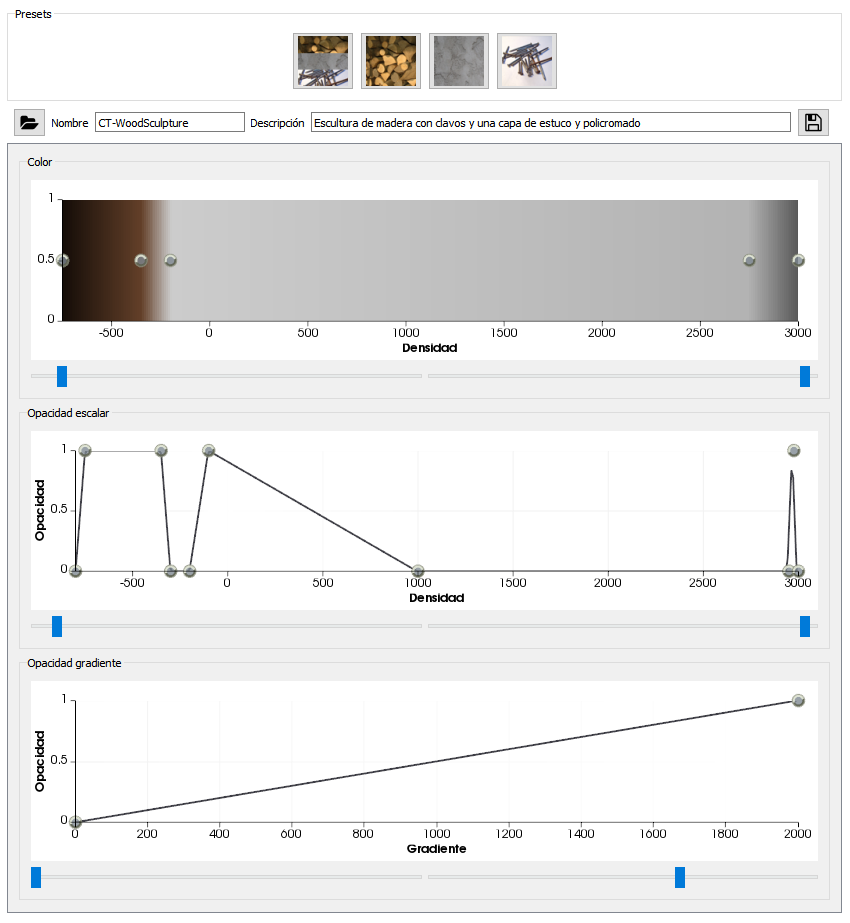
\includegraphics[width=9cm]{imagenes/pestana_funcion_de_transferencia}
	\caption{Pestaña de la GUI donde se puede modificar la función de transferencia}
	\label{fig:pestana_funcion_de_transferencia}
\end{figure}

Desde la GUI (Figura \ref{fig:pestana_funcion_de_transferencia}) además de tener las gráficas y los botones para cambiar de preset se puede importar una función de transferencia o exportar la que se esté usando en ese momento para poder utilizarla en cualquier otro momento o compartirla con otros usuarios.

\section{Plano de corte}

Para interactuar con el plano hay que hacer click derecho sobre éste y moverlo. Para girarlo hay que hacer el click derecho en los bordes de éste. Además desde la GUI (Figura \ref{fig:gui_plano}) se puede cambiar a posiciones por defecto del plano (rojo: sagital, verde: axial y azul: coronal), guardar una imagen del corte y activar o desactivar el plano para que no se muestre en el visor de la reconstrucción volumétrica en 3D.

\begin{figure}[H]
	\centering
	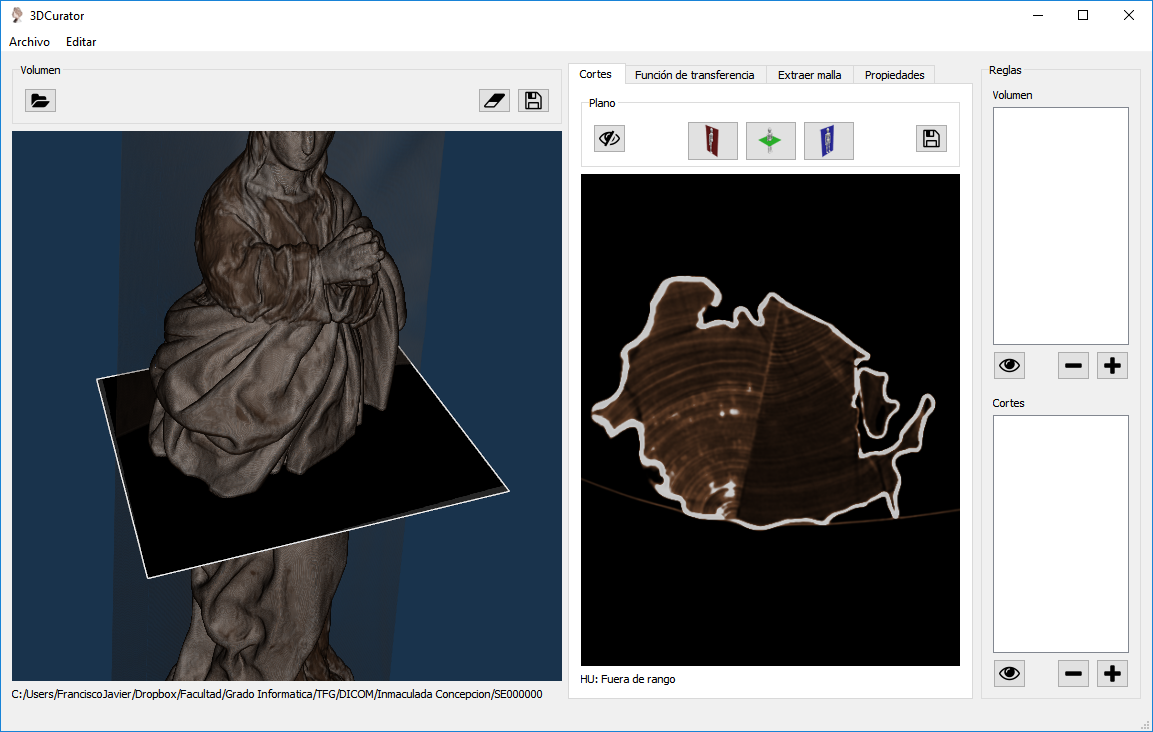
\includegraphics[width=12.5cm]{imagenes/gui_plano}
	\caption{GUI completa con la pestaña del plano activa donde se puede ver el corte que produce el plano oblicuo en la escultura}
	\label{fig:gui_plano}
\end{figure}

La visualización de cortes es tal vez la funcionalidad más útil para un restaurador y es que puede ver el interior de la figura sin tener que dañarla.

En el caso de la Inmaculada Concepción, por ejemplo, en la zona inferior (Figura \ref{fig:corte_inmaculada_concepcion_agujero}) se pueden apreciar hasta cinco piezas de madera distintas: las dos principales base de la escultura,  dos en los laterales y una frontal en la que está la cabeza de un ángel esculpido. Además en este corte se aprecia menos cantidad de estuco que en las zonas donde se encuentra el manto. Se puede observar también el agujero en el centro utilizado para colocar la figura así como los anillos de la madera, útil para determinar la edad de ésta.

\begin{figure}[H]
	\centering
	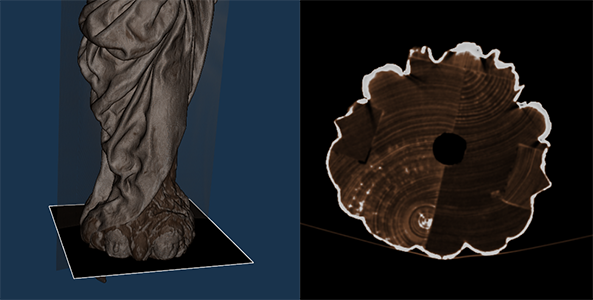
\includegraphics[width=12.5cm]{imagenes/corte_inmaculada_concepcion_agujero}
	\caption{Corte en la zona inferior de la escultura de Inmaculada Concepción}
	\label{fig:corte_inmaculada_concepcion_agujero}
\end{figure}

Examinando la escultura de San Juan Evangelista, también en la zona inferior (Figura \ref{fig:corte_san_juan_evangelista_clavos_pies}) se pueden observar un par de piezas de madera y los dos clavos de los pies.

\begin{figure}[H]
	\centering
	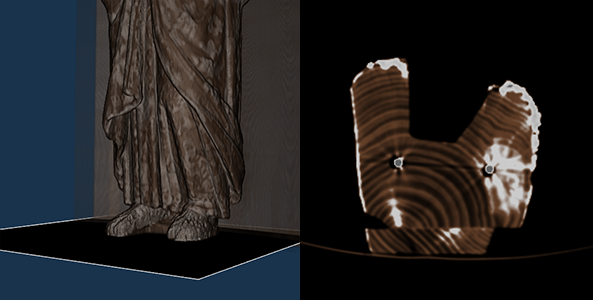
\includegraphics[width=12.5cm]{imagenes/corte_san_juan_evangelista_clavos_pies}
	\caption{Corte en la zona inferior de la escultura de San Juan Evangelista}
	\label{fig:corte_san_juan_evangelista_clavos_pies}
\end{figure}

En el corte anterior se puede ver algo de distorsión producida por el metal, pero donde mejor se puede observar este fenómeno es en el clavo del centro donde parece que hay una zona hueca y otra rellena de estuco, pero realmente estas zonas tienen estos valores por culpa del ruido que produce el clavo durante el escaneo.

\begin{figure}[H]
	\centering
	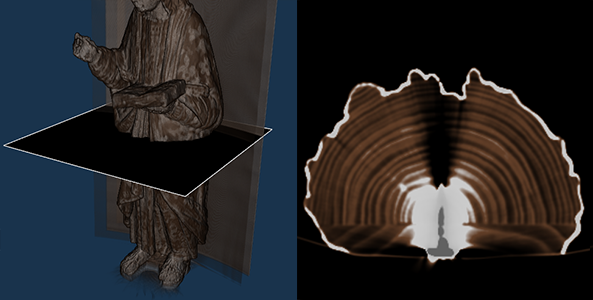
\includegraphics[width=12.5cm]{imagenes/corte_san_juan_evangelista_clavo}
	\caption{Corte en la zona central de la escultura de San Juan Evangelista donde se encuentra el clavo}
	\label{fig:corte_san_juan_evangelista_clavo}
\end{figure}

\section{Reglas}

Lalala

\section{Extraer malla}

Lalala
